\documentclass[aspectratio=169,10pt]{beamer}
\usepackage[T1]{fontenc}
\usepackage[scaled=0.9]{helvet}   % stand-in for Amazon Ember (not installed)
\renewcommand{\familydefault}{\sfdefault}
\usepackage{booktabs,tabularx,multirow,makecell,colortbl,xcolor}
\usepackage{graphicx}
\usepackage{pgfplots}
\pgfplotsset{compat=1.18}
\usepackage{listings}
\usepackage{fontawesome5}

% ---- AWS template palette (dark) ----------------------------------
\definecolor{bgdark}{HTML}{161D26}
\definecolor{panel}{HTML}{232F3E}
\definecolor{awsblue}{HTML}{007DFF}
\definecolor{awspurple}{HTML}{952EFF}
\definecolor{awsmagenta}{HTML}{E433FF}
\definecolor{awsteal}{HTML}{00D6C7}
\definecolor{bodytext}{HTML}{F2F4F7}
\definecolor{inkmuted}{HTML}{A3ACB9}
\definecolor{footc}{HTML}{8B95A3}
\definecolor{rulec}{HTML}{5A6573}
\definecolor{gridc}{HTML}{333E4C}
\definecolor{vendorc}{HTML}{7B8594}
\definecolor{linkc}{HTML}{5FB0FF}
\definecolor{sectag}{HTML}{E433FF}
% extra categorical colours for charts, tuned for the dark background
\definecolor{cat1}{HTML}{EB6834}   % orange
\definecolor{cat2}{HTML}{3B8BEB}   % blue
\definecolor{cat3}{HTML}{1BAF7A}   % aqua

% footer text; override with \renewcommand{\deckfooter}{...} after \documentclass[aspectratio=169,10pt]{beamer}
\usepackage[T1]{fontenc}
\usepackage[scaled=0.9]{helvet}   % stand-in for Amazon Ember (not installed)
\renewcommand{\familydefault}{\sfdefault}
\usepackage{booktabs,tabularx,multirow,makecell,colortbl,xcolor}
\usepackage{graphicx}
\usepackage{pgfplots}
\pgfplotsset{compat=1.18}
\usepackage{listings}
\usepackage{fontawesome5}

% ---- AWS template palette (dark) ----------------------------------
\definecolor{bgdark}{HTML}{161D26}
\definecolor{panel}{HTML}{232F3E}
\definecolor{awsblue}{HTML}{007DFF}
\definecolor{awspurple}{HTML}{952EFF}
\definecolor{awsmagenta}{HTML}{E433FF}
\definecolor{awsteal}{HTML}{00D6C7}
\definecolor{bodytext}{HTML}{F2F4F7}
\definecolor{inkmuted}{HTML}{A3ACB9}
\definecolor{footc}{HTML}{8B95A3}
\definecolor{rulec}{HTML}{5A6573}
\definecolor{gridc}{HTML}{333E4C}
\definecolor{vendorc}{HTML}{7B8594}
\definecolor{linkc}{HTML}{5FB0FF}
\definecolor{sectag}{HTML}{E433FF}
% extra categorical colours for charts, tuned for the dark background
\definecolor{cat1}{HTML}{EB6834}   % orange
\definecolor{cat2}{HTML}{3B8BEB}   % blue
\definecolor{cat3}{HTML}{1BAF7A}   % aqua

% footer text; override with \renewcommand{\deckfooter}{...} after \documentclass[aspectratio=169,10pt]{beamer}
\usepackage[T1]{fontenc}
\usepackage[scaled=0.9]{helvet}   % stand-in for Amazon Ember (not installed)
\renewcommand{\familydefault}{\sfdefault}
\usepackage{booktabs,tabularx,multirow,makecell,colortbl,xcolor}
\usepackage{graphicx}
\usepackage{pgfplots}
\pgfplotsset{compat=1.18}
\usepackage{listings}
\usepackage{fontawesome5}

% ---- AWS template palette (dark) ----------------------------------
\definecolor{bgdark}{HTML}{161D26}
\definecolor{panel}{HTML}{232F3E}
\definecolor{awsblue}{HTML}{007DFF}
\definecolor{awspurple}{HTML}{952EFF}
\definecolor{awsmagenta}{HTML}{E433FF}
\definecolor{awsteal}{HTML}{00D6C7}
\definecolor{bodytext}{HTML}{F2F4F7}
\definecolor{inkmuted}{HTML}{A3ACB9}
\definecolor{footc}{HTML}{8B95A3}
\definecolor{rulec}{HTML}{5A6573}
\definecolor{gridc}{HTML}{333E4C}
\definecolor{vendorc}{HTML}{7B8594}
\definecolor{linkc}{HTML}{5FB0FF}
\definecolor{sectag}{HTML}{E433FF}
% extra categorical colours for charts, tuned for the dark background
\definecolor{cat1}{HTML}{EB6834}   % orange
\definecolor{cat2}{HTML}{3B8BEB}   % blue
\definecolor{cat3}{HTML}{1BAF7A}   % aqua

% footer text; override with \renewcommand{\deckfooter}{...} after \input{preamble}
\newcommand{\deckfooter}{\textcopyright{} \the\year, Amazon Web Services, Inc. or its affiliates.}

% ---- beamer look ---------------------------------------------------
\setbeamercolor{background canvas}{bg=bgdark}
\setbeamercolor{normal text}{fg=bodytext,bg=bgdark}
\setbeamercolor{structure}{fg=awsblue}
\setbeamercolor{frametitle}{fg=white}
\setbeamercolor{itemize item}{fg=awsteal}
\setbeamercolor{itemize subitem}{fg=inkmuted}
\setbeamercolor{enumerate item}{fg=awsteal}
\setbeamercolor{alerted text}{fg=awsmagenta}
\setbeamertemplate{navigation symbols}{}
\setbeamertemplate{itemize items}[square]
\setbeamertemplate{enumerate items}[default]
\setbeamertemplate{caption}[numbered]
\setbeamerfont{itemize/enumerate subbody}{size=\scriptsize}
\setbeamersize{text margin left=8mm,text margin right=8mm}

% section tag shown above each frame title (no divider slides)
\gdef\secname{}
\newcommand{\sect}[1]{\section{#1}\gdef\secname{#1}}
\setbeamertemplate{frametitle}{%
  \nointerlineskip\vskip3.2mm
  \ifx\secname\empty\else{\fontsize{6.5}{7}\selectfont\bfseries\color{sectag}\MakeUppercase{\secname}}\par\vskip0.9mm\fi
  {\fontsize{12.5}{14.5}\selectfont\bfseries\color{white}\insertframetitle}\par\vskip0.6mm}
\setbeamertemplate{headline}{}
\setbeamertemplate{footline}{%
  \hbox to\paperwidth{\hspace*{8mm}{\fontsize{5}{6}\selectfont\color{footc}\deckfooter}\hfill{\fontsize{6}{7}\selectfont\color{footc}\insertframenumber}\hspace*{8mm}}\vskip2.5mm}

% ---- deck macros ---------------------------------------------------
\newcommand{\hl}[1]{\textcolor{awsteal}{\textbf{#1}}}
\newcommand{\src}[1]{\vfill{\tiny\textcolor{footc}{Source: #1}}}
\newcommand{\flabel}[1]{\label{#1}\hypertarget{#1}{}}
% clickable slide references
\newcommand{\sref}[1]{\hyperlink{#1}{\textcolor{linkc}{slide~\pageref*{#1}}}}
\newcommand{\srefs}[2]{\textcolor{linkc}{slides~\hyperlink{#1}{\pageref*{#1}}--\hyperlink{#2}{\pageref*{#2}}}}
\newcommand{\plainen}[1]{\colorbox{panel}{\parbox{\dimexpr\linewidth-2\fboxsep}{\raggedright\footnotesize\textbf{In plain English:} #1}}\par\vspace{1mm}}
\newcommand{\idcard}[1]{\colorbox{panel}{\parbox{\dimexpr\textwidth-2\fboxsep}{\scriptsize #1}}}
\newcommand{\grp}[2]{\multicolumn{#1}{@{}l}{\textcolor{awsteal}{\textit{#2}}}}
\newcommand{\agi}[4]{\hyperlink{#1}{{\large\bfseries\color{awsteal}#2}\quad{\large\bfseries\color{white}#3}}\\[0.5mm]{\small\color{inkmuted}#4}\par\vspace{4mm}}
\newcommand{\bgframe}[1]{\usebackgroundtemplate{\includegraphics[width=\paperwidth,height=\paperheight]{#1}}}

\arrayrulecolor{rulec}
\lstset{basicstyle=\ttfamily\tiny\color{bodytext},breaklines=true,columns=fullflexible,
  backgroundcolor=\color{panel},frame=single,rulecolor=\color{rulec},
  keywordstyle=\color{awsteal}\bfseries,commentstyle=\color{inkmuted},showstringspaces=false}
\renewcommand{\arraystretch}{1.1}
\usetikzlibrary{arrows.meta,positioning,shapes.geometric,calc,fit,backgrounds,shadows}
\tikzset{box/.style={draw=awsblue,fill=panel,rounded corners=2pt,align=center,font=\scriptsize,inner sep=3pt,text=bodytext},
         arr/.style={-{Stealth[length=2mm]},thick,awsblue}}
\pgfplotsset{every axis/.append style={axis line style={rulec},tick style={rulec},
  tick label style={text=bodytext},label style={text=bodytext}}}

% numbered table / figure labels (one index across the deck)
\newcounter{tabno}\newcounter{figno}
\newcommand{\tabcap}[1]{\refstepcounter{tabno}{\scriptsize\bfseries\color{awsteal}Table~\thetabno\hspace{0.6em}{\color{bodytext}#1}}\par\vspace{0.2mm}}
\newcommand{\figcap}[1]{\refstepcounter{figno}{\scriptsize\bfseries\color{awsteal}Figure~\thefigno\hspace{0.6em}{\color{bodytext}#1}}\par\vspace{0.2mm}}

% ---- project additions ----------------------------------------------
% A light-background figure (existing diagrams/plots) shown on a white card so it reads on the dark theme.
\newcommand{\figcard}[2][]{{\setlength{\fboxsep}{2mm}\colorbox{white}{\includegraphics[#1]{#2}}}}
\graphicspath{{../figures/}}

\newcommand{\deckfooter}{\textcopyright{} \the\year, Amazon Web Services, Inc. or its affiliates.}

% ---- beamer look ---------------------------------------------------
\setbeamercolor{background canvas}{bg=bgdark}
\setbeamercolor{normal text}{fg=bodytext,bg=bgdark}
\setbeamercolor{structure}{fg=awsblue}
\setbeamercolor{frametitle}{fg=white}
\setbeamercolor{itemize item}{fg=awsteal}
\setbeamercolor{itemize subitem}{fg=inkmuted}
\setbeamercolor{enumerate item}{fg=awsteal}
\setbeamercolor{alerted text}{fg=awsmagenta}
\setbeamertemplate{navigation symbols}{}
\setbeamertemplate{itemize items}[square]
\setbeamertemplate{enumerate items}[default]
\setbeamertemplate{caption}[numbered]
\setbeamerfont{itemize/enumerate subbody}{size=\scriptsize}
\setbeamersize{text margin left=8mm,text margin right=8mm}

% section tag shown above each frame title (no divider slides)
\gdef\secname{}
\newcommand{\sect}[1]{\section{#1}\gdef\secname{#1}}
\setbeamertemplate{frametitle}{%
  \nointerlineskip\vskip3.2mm
  \ifx\secname\empty\else{\fontsize{6.5}{7}\selectfont\bfseries\color{sectag}\MakeUppercase{\secname}}\par\vskip0.9mm\fi
  {\fontsize{12.5}{14.5}\selectfont\bfseries\color{white}\insertframetitle}\par\vskip0.6mm}
\setbeamertemplate{headline}{}
\setbeamertemplate{footline}{%
  \hbox to\paperwidth{\hspace*{8mm}{\fontsize{5}{6}\selectfont\color{footc}\deckfooter}\hfill{\fontsize{6}{7}\selectfont\color{footc}\insertframenumber}\hspace*{8mm}}\vskip2.5mm}

% ---- deck macros ---------------------------------------------------
\newcommand{\hl}[1]{\textcolor{awsteal}{\textbf{#1}}}
\newcommand{\src}[1]{\vfill{\tiny\textcolor{footc}{Source: #1}}}
\newcommand{\flabel}[1]{\label{#1}\hypertarget{#1}{}}
% clickable slide references
\newcommand{\sref}[1]{\hyperlink{#1}{\textcolor{linkc}{slide~\pageref*{#1}}}}
\newcommand{\srefs}[2]{\textcolor{linkc}{slides~\hyperlink{#1}{\pageref*{#1}}--\hyperlink{#2}{\pageref*{#2}}}}
\newcommand{\plainen}[1]{\colorbox{panel}{\parbox{\dimexpr\linewidth-2\fboxsep}{\raggedright\footnotesize\textbf{In plain English:} #1}}\par\vspace{1mm}}
\newcommand{\idcard}[1]{\colorbox{panel}{\parbox{\dimexpr\textwidth-2\fboxsep}{\scriptsize #1}}}
\newcommand{\grp}[2]{\multicolumn{#1}{@{}l}{\textcolor{awsteal}{\textit{#2}}}}
\newcommand{\agi}[4]{\hyperlink{#1}{{\large\bfseries\color{awsteal}#2}\quad{\large\bfseries\color{white}#3}}\\[0.5mm]{\small\color{inkmuted}#4}\par\vspace{4mm}}
\newcommand{\bgframe}[1]{\usebackgroundtemplate{\includegraphics[width=\paperwidth,height=\paperheight]{#1}}}

\arrayrulecolor{rulec}
\lstset{basicstyle=\ttfamily\tiny\color{bodytext},breaklines=true,columns=fullflexible,
  backgroundcolor=\color{panel},frame=single,rulecolor=\color{rulec},
  keywordstyle=\color{awsteal}\bfseries,commentstyle=\color{inkmuted},showstringspaces=false}
\renewcommand{\arraystretch}{1.1}
\usetikzlibrary{arrows.meta,positioning,shapes.geometric,calc,fit,backgrounds,shadows}
\tikzset{box/.style={draw=awsblue,fill=panel,rounded corners=2pt,align=center,font=\scriptsize,inner sep=3pt,text=bodytext},
         arr/.style={-{Stealth[length=2mm]},thick,awsblue}}
\pgfplotsset{every axis/.append style={axis line style={rulec},tick style={rulec},
  tick label style={text=bodytext},label style={text=bodytext}}}

% numbered table / figure labels (one index across the deck)
\newcounter{tabno}\newcounter{figno}
\newcommand{\tabcap}[1]{\refstepcounter{tabno}{\scriptsize\bfseries\color{awsteal}Table~\thetabno\hspace{0.6em}{\color{bodytext}#1}}\par\vspace{0.2mm}}
\newcommand{\figcap}[1]{\refstepcounter{figno}{\scriptsize\bfseries\color{awsteal}Figure~\thefigno\hspace{0.6em}{\color{bodytext}#1}}\par\vspace{0.2mm}}

% ---- project additions ----------------------------------------------
% A light-background figure (existing diagrams/plots) shown on a white card so it reads on the dark theme.
\newcommand{\figcard}[2][]{{\setlength{\fboxsep}{2mm}\colorbox{white}{\includegraphics[#1]{#2}}}}
\graphicspath{{../figures/}}

\newcommand{\deckfooter}{\textcopyright{} \the\year, Amazon Web Services, Inc. or its affiliates.}

% ---- beamer look ---------------------------------------------------
\setbeamercolor{background canvas}{bg=bgdark}
\setbeamercolor{normal text}{fg=bodytext,bg=bgdark}
\setbeamercolor{structure}{fg=awsblue}
\setbeamercolor{frametitle}{fg=white}
\setbeamercolor{itemize item}{fg=awsteal}
\setbeamercolor{itemize subitem}{fg=inkmuted}
\setbeamercolor{enumerate item}{fg=awsteal}
\setbeamercolor{alerted text}{fg=awsmagenta}
\setbeamertemplate{navigation symbols}{}
\setbeamertemplate{itemize items}[square]
\setbeamertemplate{enumerate items}[default]
\setbeamertemplate{caption}[numbered]
\setbeamerfont{itemize/enumerate subbody}{size=\scriptsize}
\setbeamersize{text margin left=8mm,text margin right=8mm}

% section tag shown above each frame title (no divider slides)
\gdef\secname{}
\newcommand{\sect}[1]{\section{#1}\gdef\secname{#1}}
\setbeamertemplate{frametitle}{%
  \nointerlineskip\vskip3.2mm
  \ifx\secname\empty\else{\fontsize{6.5}{7}\selectfont\bfseries\color{sectag}\MakeUppercase{\secname}}\par\vskip0.9mm\fi
  {\fontsize{12.5}{14.5}\selectfont\bfseries\color{white}\insertframetitle}\par\vskip0.6mm}
\setbeamertemplate{headline}{}
\setbeamertemplate{footline}{%
  \hbox to\paperwidth{\hspace*{8mm}{\fontsize{5}{6}\selectfont\color{footc}\deckfooter}\hfill{\fontsize{6}{7}\selectfont\color{footc}\insertframenumber}\hspace*{8mm}}\vskip2.5mm}

% ---- deck macros ---------------------------------------------------
\newcommand{\hl}[1]{\textcolor{awsteal}{\textbf{#1}}}
\newcommand{\src}[1]{\vfill{\tiny\textcolor{footc}{Source: #1}}}
\newcommand{\flabel}[1]{\label{#1}\hypertarget{#1}{}}
% clickable slide references
\newcommand{\sref}[1]{\hyperlink{#1}{\textcolor{linkc}{slide~\pageref*{#1}}}}
\newcommand{\srefs}[2]{\textcolor{linkc}{slides~\hyperlink{#1}{\pageref*{#1}}--\hyperlink{#2}{\pageref*{#2}}}}
\newcommand{\plainen}[1]{\colorbox{panel}{\parbox{\dimexpr\linewidth-2\fboxsep}{\raggedright\footnotesize\textbf{In plain English:} #1}}\par\vspace{1mm}}
\newcommand{\idcard}[1]{\colorbox{panel}{\parbox{\dimexpr\textwidth-2\fboxsep}{\scriptsize #1}}}
\newcommand{\grp}[2]{\multicolumn{#1}{@{}l}{\textcolor{awsteal}{\textit{#2}}}}
\newcommand{\agi}[4]{\hyperlink{#1}{{\large\bfseries\color{awsteal}#2}\quad{\large\bfseries\color{white}#3}}\\[0.5mm]{\small\color{inkmuted}#4}\par\vspace{4mm}}
\newcommand{\bgframe}[1]{\usebackgroundtemplate{\includegraphics[width=\paperwidth,height=\paperheight]{#1}}}

\arrayrulecolor{rulec}
\lstset{basicstyle=\ttfamily\tiny\color{bodytext},breaklines=true,columns=fullflexible,
  backgroundcolor=\color{panel},frame=single,rulecolor=\color{rulec},
  keywordstyle=\color{awsteal}\bfseries,commentstyle=\color{inkmuted},showstringspaces=false}
\renewcommand{\arraystretch}{1.1}
\usetikzlibrary{arrows.meta,positioning,shapes.geometric,calc,fit,backgrounds,shadows}
\tikzset{box/.style={draw=awsblue,fill=panel,rounded corners=2pt,align=center,font=\scriptsize,inner sep=3pt,text=bodytext},
         arr/.style={-{Stealth[length=2mm]},thick,awsblue}}
\pgfplotsset{every axis/.append style={axis line style={rulec},tick style={rulec},
  tick label style={text=bodytext},label style={text=bodytext}}}

% numbered table / figure labels (one index across the deck)
\newcounter{tabno}\newcounter{figno}
\newcommand{\tabcap}[1]{\refstepcounter{tabno}{\scriptsize\bfseries\color{awsteal}Table~\thetabno\hspace{0.6em}{\color{bodytext}#1}}\par\vspace{0.2mm}}
\newcommand{\figcap}[1]{\refstepcounter{figno}{\scriptsize\bfseries\color{awsteal}Figure~\thefigno\hspace{0.6em}{\color{bodytext}#1}}\par\vspace{0.2mm}}

% ---- project additions ----------------------------------------------
% A light-background figure (existing diagrams/plots) shown on a white card so it reads on the dark theme.
\newcommand{\figcard}[2][]{{\setlength{\fboxsep}{2mm}\colorbox{white}{\includegraphics[#1]{#2}}}}
\graphicspath{{../figures/}}

\usepackage{amssymb}
\usepackage{tabularx}
\newcommand{\yes}{\textcolor{awsteal}{$\checkmark$}}
\definecolor{armnone}{HTML}{D9591A}
\newcommand{\no}{\textcolor{awsmagenta}{$\times$}}

\title{SWE-bench on AgentCore}
\author{Kaige Yang}
\institute{Senior Applied Scientist, AWS}
\date{September 2026}

\begin{document}

%====================================================================
{\bgframe{art/bg_title.jpg}
\begin{frame}[plain]
\vspace*{6mm}
\begin{minipage}{0.56\textwidth}
{\fontsize{26}{30}\selectfont\bfseries\color{white}SWE-bench on\\AgentCore\par}
\vspace{4mm}
{\raggedright\large\color{white}Image sizes, the arm64 and 2\,GB limits, and three sandbox demos for agentic RL: AgentCore, EKS, ECS\par}
\vspace{12mm}
{\small\color{white}\textbf{Kaige Yang}\\Senior Applied Scientist, AWS\par}
\vspace{3mm}
{\scriptsize\color{inkmuted}Data as of September 28, 2026}
\end{minipage}
\end{frame}}

%====================================================================
\begin{frame}
\flabel{fr:agenda}
\vspace*{2mm}
\begin{columns}[c]
\column{0.28\textwidth}
{\fontsize{24}{28}\selectfont\bfseries\color{white}Agenda}
\column{0.04\textwidth}
\tikz\fill[awsmagenta] (0,0) rectangle (0.6pt,62mm);
\column{0.64\textwidth}
\agi{fr:task}{01}{Background}{What an SWE-bench task needs from a sandbox}
\agi{fr:limits}{02}{Survey}{All 500 Verified images vs the AgentCore limits, probed on AWS}
\agi{fr:ch1}{03}{Challenges and solutions}{arm64, the 2\,GB cap, and a two-lane design}
\agi{fr:built}{04}{What we built}{AgentCore (first run, arm64), EKS + gVisor, ECS: limits of each, compared}
{\scriptsize\color{footc}Appendix (\hyperlink{fr:appx}{\textcolor{linkc}{from slide~\pageref*{fr:appx}}}): per-repo detail and references.}
\end{columns}
\end{frame}

%====================================================================
\begin{frame}{Most SWE-bench rows qualify for AgentCore microVMs on architecture and size; an m5 lane covers the tail}
\flabel{fr:summary}
\footnotesize
\begin{tabularx}{\textwidth}{@{}>{\bfseries\raggedright\arraybackslash}p{2.3cm}X@{}}
\toprule
Goal & RL-train a coding agent (Qwen3-4B, slime GRPO) on \hl{SWE-bench}, each episode in its own isolated AgentCore sandbox.\\
Background & SWE-bench needs \textbf{one image per dataset row} (repo + commit + environment); the official images are amd64, p50 1.08\,GB compressed.\\
Limits, probed & The 2\,GB cap counts the \textbf{compressed} size and is enforced when the Runtime is created (\hl{2048\,MiB}: 2,042 accepted, 2,062 rejected; 3\,GB on disk / 64\,MB compressed accepted). Cold open 22--30\,s at 1.5--2\,GiB; $\approx$\,10 pre-warmed per new Runtime.\\
arm64 & microVMs are arm64-only, but \textbf{prebuilt arm64 images exist for \hl{420 / 500} rows}, all $\le$ 2\,GB (Epoch AI on GHCR; 281 also official) (\sref{fr:arm64}).\\
Solutions & Re-wrap the existing arm64 images, rebuild the rest per (repo, version) environment, slim what's over 2\,GB, and route the remaining rows to an \textbf{m5 Instance lane}.\\
Not yet shown & No real SWE-bench image has run on a microVM yet: the 420 are \emph{eligible}, not validated. 139 of them exist only as Epoch builds, assumed to keep the official \texttt{/testbed} layout.\\
Built on AgentCore & \texttt{demo\_cpu\_swebench}, 20 tasks. First run (m5 lane): 24 episodes, \hl{0 infra errors}, the $\approx$\,90\,s boot hidden; 0 solved. Now on \textbf{arm64 microVMs}: local oracle check passes, AWS run pending (\sref{fr:armnow}).\\
EKS and ECS twins (not deployed) & Same rows, grader and amd64 images: one \textbf{gVisor pod} (\texttt{\_eks}) or one \textbf{ECS task} (\texttt{\_ecs}) per episode on shared m5 nodes; no image limits, weaker boundaries (\sref{fr:cmp3}).\\
\bottomrule
\end{tabularx}
\src{\texttt{code/demos/demo\_cpu\_swebench/} (\texttt{survey\_image\_sizes.py}, \texttt{probe\_image\_cap.py}, smoke log 2026-09-28); checked 2026-09-28.}
\end{frame}

%====================================================================
\sect{Background}

%====================================================================
\begin{frame}{Every SWE-bench row is its own repo, commit and environment, so one image can't serve the dataset}
\flabel{fr:task}
\begin{columns}[T]
\column{0.56\textwidth}
\tabcap{The task}
\scriptsize
\begin{tabularx}{\linewidth}{@{}>{\bfseries}p{1.7cm}X@{}}
\toprule
Input & A real GitHub issue + the repo checked out at \texttt{base\_commit}, dependencies installed\\
Agent's job & Explore, edit, run code: a multi-turn tool loop (\texttt{bash} / \texttt{read\_file} / \texttt{write\_file})\\
Reward (RLVR) & Hidden \texttt{test\_patch} applied \textbf{after} the agent stops; solved iff every FAIL\_TO\_PASS and PASS\_TO\_PASS test passes. No LLM judge\\
Verified & \textbf{500} human-validated instances from \textbf{12} Python repos\\
Training scale & Full test set 2,294; SWE-Gym \textbf{2,438}; SWE-smith \textbf{59,136}; same per-instance format\\
\bottomrule
\end{tabularx}
\column{0.40\textwidth}
\begin{itemize}\footnotesize\setlength{\itemsep}{1.5mm}
\item \textbf{A sandbox problem:} each row has a different repo, commit and dependency set. The official harness ships one prebuilt image per instance, \texttt{swebench/sweb.eval.x86\_64.<id>}.
\item \textbf{RL adds scale:} NS GRPO siblings per task per step, each in a \hl{pristine} copy of the environment, thousands of episodes per run.
\end{itemize}
\plainen{every exercise comes with its own computer, and each attempt needs a clean copy of it.}
\end{columns}
\src{\texttt{princeton-nlp/SWE-bench\_Verified}, \texttt{SWE-Gym/SWE-Gym} (train 2,438), \texttt{SWE-bench/SWE-smith} (train 59,136) on Hugging Face; checked 2026-09-28.}
\end{frame}

%====================================================================
\begin{frame}{Each episode needs the row's exact environment, a fresh machine and a route back to the trainer}
\flabel{fr:needs}
\tabcap{What the sandbox must provide per episode}
\scriptsize
\begin{tabularx}{\textwidth}{@{}>{\bfseries}p{3.2cm}XX@{}}
\toprule
Need & Why & AgentCore mechanism\\
\midrule
The row's exact environment & Tests only mean something in the environment SWE-bench validated & A custom image per row (or per environment) $\rightarrow$ Runtime\\
Fresh state every episode & The agent edits files and installs packages; GRPO siblings must not see each other & One brand-new \texttt{runtimeSessionId} = a fresh microVM or instance\\
Minutes of tool calls + a test run & Our grader allows each test run up to 600\,s & 15-minute request timeout; heartbeat past the idle timeout\\
A route back to the policy & The agent loop runs \textbf{in} the session and calls the trainer & VPC mode, SG$\rightarrow$SG rule to the adapter ports\\
Hidden tests & Stops reward hacking & \texttt{test\_patch} lives only on the trainer, injected at grading\\
\bottomrule
\end{tabularx}
\par\vspace{3mm}
{\small\raggedright\hl{Takeaway}: AgentCore already has every mechanism; the open questions are the image (arm64, size), not the session model.\par}
\src{AgentCore developer guide [D1] and quotas [Q1]; project design in \texttt{demo\_cpu\_swebench}; checked 2026-09-28.}
\end{frame}

%====================================================================
\begin{frame}{500 Verified rows collapse to 80 environments, and django alone is 46\,\% of them}
\flabel{fr:dataset}
\begin{columns}[T]
\column{0.56\textwidth}
\tabcap{SWE-bench Verified by repo (500 instances)}
\scriptsize\setlength{\tabcolsep}{4pt}
\begin{tabular}{@{}lrr@{\hspace{8mm}}lrr@{}}
\toprule
\textbf{Repo} & \textbf{Inst.} & \textbf{Vers.} & \textbf{Repo} & \textbf{Inst.} & \textbf{Vers.}\\
\midrule
django & \hl{231} & 9 & astropy & 22 & 6\\
sympy & 75 & 12 & xarray & 22 & 4\\
sphinx & 44 & 15 & pytest & 19 & 10\\
matplotlib & 34 & 6 & pylint & 10 & 5\\
scikit-learn & 32 & 4 & requests & 8 & 7\\
seaborn & 2 & 1 & flask & 1 & 1\\
\midrule
\multicolumn{3}{@{}l}{\textbf{Total}} & & \textbf{500} & \textbf{80}\\
\bottomrule
\end{tabular}
\column{0.40\textwidth}
\begin{itemize}\footnotesize\setlength{\itemsep}{1.5mm}
\item \textbf{Only 80 distinct (repo, version) environments.} Instances of one environment differ only in the commit checked out.
\item That makes \hl{one image per environment} possible: 500 $\rightarrow$ 80 images and Runtimes (\sref{fr:ch2}).
\end{itemize}
\end{columns}
\src{\texttt{princeton-nlp/SWE-bench\_Verified} (test split), grouped by \texttt{repo} and \texttt{version}; checked 2026-09-28.}
\end{frame}

%====================================================================
\sect{Survey}

%====================================================================
\begin{frame}{Two microVM limits matter: arm64 only, and a 2\,GB image cap that can't be raised}
\flabel{fr:limits}
\begin{columns}[T]
\column{0.56\textwidth}
\tabcap{The AgentCore limits that matter}
\scriptsize
\begin{tabularx}{\linewidth}{@{}Xlc@{}}
\toprule
\textbf{Limit} & \textbf{Value} & \textbf{Ref}\\
\midrule
microVM CPU architecture & \hl{arm64 only} & [D1]\\
Max image size (L-0A9E32B3) & \hl{2048\,MiB compressed, not adjustable} & [Q2][P1]\\
Runtimes per account & 1000 & [Q1]\\
Active / new sessions & 5000 / 25 per s & [Q2]\\
Capacity-provider Instances (m5, g6) & amd64, no 2\,GB cap & [D2]\\
\bottomrule
\end{tabularx}
\column{0.40\textwidth}
\begin{itemize}\footnotesize\setlength{\itemsep}{1.5mm}
\item The quota text says ``maximum container size'' without saying compressed or on disk, so \textbf{we probed it on AWS} (\sref{fr:capprobe}).
\item Instances have no cap and run amd64, but \textbf{1 session = 1 instance}: a whole m5 per episode.
\end{itemize}
\end{columns}
\src{\texttt{aws service-quotas get-service-quota --service-code bedrock-agentcore} (us-west-2) [Q2]; AgentCore docs [Q1][D1]; project measurement [D2]; checked 2026-09-28.}
\end{frame}

%====================================================================
\begin{frame}{The cap is 2048\,MiB of compressed image, enforced when the Runtime is created}
\flabel{fr:capprobe}
\begin{columns}[T]
\column{0.56\textwidth}
\tabcap{Cap probe: one 61\,MiB base image + a filler layer, arm64, VPC mode}
\scriptsize\setlength{\tabcolsep}{3pt}
\begin{tabular}{@{}lrrl@{}}
\toprule
\textbf{Filler} & \textbf{Compressed} & \textbf{Create} & \textbf{Sessions}\\
\midrule
3\,GiB zeros (3.1\,GiB on disk) & 64\,MiB & \hl{READY} & 5/5\\
1,000\,MiB random & 1,061\,MiB & READY & 5/5\\
1,500\,MiB random & 1,562\,MiB & READY & 5/5\\
1,890\,MiB random & 1,952\,MiB & READY & 13/13\\
1,940\,MiB random & 2,002\,MiB & READY & 13/13\\
1,980\,MiB random & \hl{2,042\,MiB} & \hl{READY} & 13/13\\
2,000\,MiB random & \textbf{2,062\,MiB} & \textcolor{awsmagenta}{\textbf{rejected}} & ---\\
2,300\,MiB random & 2,362\,MiB & \textcolor{awsmagenta}{\textbf{rejected}} & ---\\
\bottomrule
\end{tabular}
\par\vspace{2mm}
{\scriptsize\color{inkmuted}Rejection: \texttt{ServiceQuotaExceededException: maxImageSizeMb limit exceeded}, returned synchronously by \texttt{CreateAgentRuntime}. MiB = $2^{20}$ bytes of ECR \texttt{imageSizeInBytes}.\par}
\column{0.40\textwidth}
\begin{itemize}\footnotesize\setlength{\itemsep}{1.5mm}
\item \textbf{Compressed, not on disk:} 3.1\,GiB on disk passes when it compresses to 64\,MiB.
\item \textbf{Binary, not decimal:} 2,042\,MiB (2.14\,GB decimal) passes, 2,062\,MiB fails, so the limit sits in (2,042, 2,062] MiB, consistent with 2048\,MiB.
\item \textbf{Budget:} our wrapper adds 54\,MiB, so a source image must be $\le$ $\approx$\,1,990\,MiB. The largest arm64 image (1,772\,MiB) has 220\,MiB spare.
\item \textbf{Fails fast} at create time, so a deploy script sees it at once.
\end{itemize}
\end{columns}
\src{\texttt{probe\_image\_cap.py} $\rightarrow$ \texttt{swebench/capprobe.csv}, \texttt{capprobe\_edge.csv}; us-west-2, two runs 2026-09-28.}
\end{frame}

%====================================================================
\begin{frame}{Near the cap a cold open takes 28--30\,s, but about 10 opens per new Runtime find a microVM already running}
\flabel{fr:boot}
\begin{columns}[T]
\column{0.54\textwidth}
\tabcap{Session open times from the cap probes (54 opens)}
\scriptsize\setlength{\tabcolsep}{4pt}
\begin{tabular}{@{}rrrrr@{}}
\toprule
\textbf{Image} & \textbf{Opens} & \textbf{Cold} & \textbf{Warm open} & \textbf{Cold open (pull+boot)}\\
\midrule
64\,MiB & 5 & 0 & 0.43--0.56\,s & ---\\
1,061\,MiB & 5 & 0 & 0.44--0.59\,s & ---\\
1,562\,MiB & 5 & 1 & 0.55--0.67\,s & 23.5\,s (22.1)\\
1,952\,MiB & 13 & 3 & 0.63--0.89\,s & 27.8--27.9\,s (27.1--27.5)\\
2,002\,MiB & 13 & 3 & 0.48--0.95\,s & 29.9--30.0\,s (28.1--28.2)\\
2,042\,MiB & 13 & 3 & 0.55--1.01\,s & 29.9--30.0\,s (28.2--28.3)\\
\bottomrule
\end{tabular}
\column{0.42\textwidth}
\begin{itemize}\footnotesize\setlength{\itemsep}{1.5mm}
\item \textbf{Warm:} the server had started before the open was sent, so AgentCore \emph{appears} to pre-warm microVMs for a new Runtime (inferred, not documented).
\item \textbf{Depth $\approx$\,10:} 1 open then a burst of 12 gave exactly 10 warm + 3 cold on all three Runtimes. Refill under sustained load is not measured.
\item \textbf{Cold:} 22\,s at 1.5\,GiB, 28--30\,s near 2\,GiB (n = 10), still \hl{$\approx$\,3$\times$ faster} than the $\approx$\,90\,s m5 boot (\sref{fr:smoke}).
\end{itemize}
\end{columns}
\src{\texttt{probe\_image\_cap.py}: 1 open, then a burst of 4 (first run) or 12 (edge run) per Runtime; warm = server started before the open was sent; us-west-2, 2026-09-28.}
\end{frame}

%====================================================================
\begin{frame}{arm64 images already exist for 420 of 500 rows, all under 2\,GB; 80 rows have none}
\flabel{fr:arm64}
\begin{columns}[T]
\column{0.55\textwidth}
\figcap{Verified rows per repo with a prebuilt arm64 image (any registry)}
\begin{tikzpicture}
\begin{axis}[xbar stacked,width=\linewidth,height=6.1cm,bar width=5.5pt,
  xmin=0,xmax=262,enlarge y limits=0.05,
  symbolic y coords={flask,seaborn,requests,pylint,pytest,xarray,astropy,scikit-learn,matplotlib,sphinx,sympy,django},
  ytick=data,yticklabels={flask 1/1,seaborn 2/2,requests 8/8,pylint 10/10,pytest 19/19,xarray 0/22,astropy 18/22,scikit-learn 7/32,matplotlib 7/34,sphinx 44/44,sympy 75/75,django 229/231},tick label style={font=\tiny},xlabel={\tiny Verified rows},
  xmajorgrids,grid style={gridc},
  legend style={font=\tiny,draw=none,fill=none,text=bodytext,at={(0.98,0.03)},anchor=south east},
  legend cell align=left]
\addplot[fill=awsblue,draw=bgdark] coordinates {(1,flask) (2,seaborn) (8,requests) (10,pylint) (19,pytest) (0,xarray) (18,astropy) (7,scikit-learn) (7,matplotlib) (44,sphinx) (75,sympy) (229,django)};
\addplot[fill=armnone,draw=bgdark] coordinates {(0,flask) (0,seaborn) (0,requests) (0,pylint) (0,pytest) (22,xarray) (4,astropy) (25,scikit-learn) (27,matplotlib) (0,sphinx) (0,sympy) (2,django)};
\legend{arm64 image (420),none (80)}
\end{axis}
\end{tikzpicture}
\column{0.41\textwidth}
\begin{itemize}\footnotesize\setlength{\itemsep}{1mm}
\item \textbf{Epoch AI (GHCR):} \hl{420 / 500} arm64, p50 0.89\,GB, max 1.73\,GB.
\item \textbf{Official (Docker Hub):} 281 / 500, all also on Epoch; p50 1.00\,GB, max 1.94\,GB.
\item \textbf{All 420 fit the cap.} Median size vs amd64: official arm64 0.92$\times$, smallest arm64 per row 0.83$\times$.
\item \textbf{Assumption:} the 139 Epoch-only rows keep the official \texttt{/testbed} + conda env \texttt{testbed} layout (not yet checked); every image still needs the oracle check (\sref{fr:ch1}).
\item \textbf{The 80 without:} matplotlib 27, scikit-learn 25, xarray 22, astropy 4, django 2 $\rightarrow$ rebuild or the m5 lane.
\end{itemize}
\end{columns}
\src{\texttt{survey\_image\_sizes.py} (Docker Hub + GHCR [S1][S2]); compressed sizes, architecture read from each image config; checked 2026-09-28. Per repo: \sref{fr:armrepo}.}
\end{frame}

%====================================================================
\begin{frame}{Every existing arm64 image fits the cap; of the 80 rows without one, 27 are over 2\,GB even on amd64}
\flabel{fr:fig1}
\figcap{Per Verified row: smallest prebuilt arm64 image (filled), or the amd64 size where none exists (hollow)}
\centering
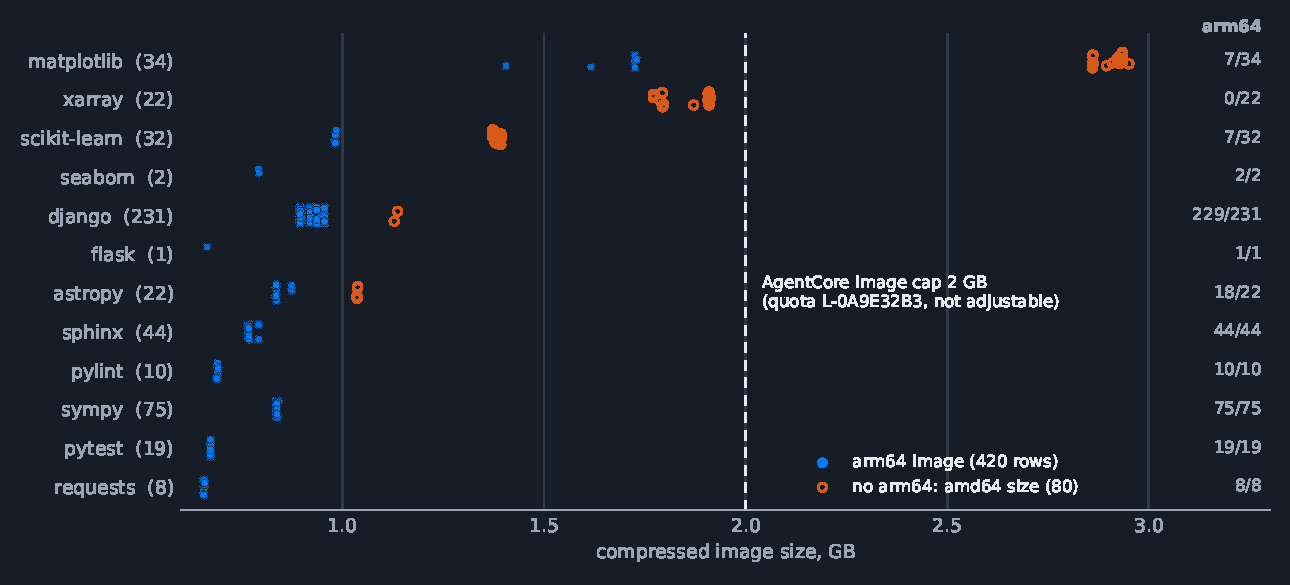
\includegraphics[height=0.60\textheight]{swe_fig03_arm64-sizes-dark.pdf}
\src{Docker Hub \texttt{swebench/sweb.eval.\{arm64,x86\_64\}.*}, GHCR \texttt{epoch-research/swe-bench.eval.arm64.*}; compressed sizes, all 500 rows (\texttt{survey\_image\_sizes.py}); checked 2026-09-28.}
\end{frame}

%====================================================================
\begin{frame}{The official amd64 images: median 1.08\,GB compressed, about 3$\times$ that on disk}
\flabel{fr:numbers}
\begin{columns}[T]
\column{0.54\textwidth}
\tabcap{Official SWE-bench Verified images (amd64, compressed)}
\scriptsize
\begin{tabularx}{\linewidth}{@{}lX@{}}
\toprule
min / p50 / p90 / max & 0.89 / \hl{1.08} / 1.79 / 2.95\,GB\\
$\le$ 1 / $\le$ 1.5 / $\le$ 2\,GB & 51 / 437 / \hl{468 of 500 (94\,\%)}\\
$>$ 2\,GB & \textbf{32, all matplotlib} (versions 3.4--3.7)\\
Total & $\approx$\,619\,GB\\
Largest repos under the cap & xarray p50 1.91\,GB, scikit-learn 1.39\,GB\\
\bottomrule
\end{tabularx}
\column{0.42\textwidth}
\begin{itemize}\footnotesize\setlength{\itemsep}{1.5mm}
\item \textbf{On disk $\approx$\,3$\times$ compressed.} Our local django image: 1.1\,GB compressed, 4.4\,GB on disk (layers 1.5 + 0.76 + 0.67 + 0.16\,GB: OS, conda, testbed env, repo).
\item \textbf{Our wrapper adds 54\,MB} (standalone Python + HTTP server), the same on all 20 images we pushed to ECR.
\item \textbf{Why amd64 still matters:} it is what the m5 lane runs (no cap), and an upper bound for arm64 rebuilds (\sref{fr:arm64}).
\end{itemize}
\end{columns}
\src{Docker Hub tags API (\texttt{survey\_image\_sizes.py}); local \texttt{docker image inspect}; ECR \texttt{describe-images} for \texttt{demo\_cpu\_swebench}; checked 2026-09-28.}
\end{frame}

%====================================================================
\begin{frame}{SWE-bench is the heavy end: about 2$\times$ as many images as Terminal-Bench, with an 8$\times$ larger median}
\flabel{fr:compare}
\tabcap{Image needs of the agentic-RL workloads we run}
\scriptsize
\begin{tabularx}{\textwidth}{@{}Xrlll@{}}
\toprule
\textbf{Workload} & \textbf{Images} & \textbf{Size p50 / max} & \textbf{arm64} & \textbf{Fits a microVM}\\
\midrule
Literature RLVR tasks (\texttt{demo\_cpu\_tasks}) & 2 & small (stdlib / + scipy) & \yes & \yes{} all\\
Terminal-Bench & 229 & 128\,MB / 6.5\,GB & built by us & 218 / 229 (7 no arm64, 4 $>$ 2\,GB)\\
\textbf{SWE-bench Verified} & \textbf{500} & \hl{1.08\,GB} / 2.95\,GB & \hl{420 / 500} prebuilt & 420 / 500 (all arm64 images $\le$ 2\,GB)\\
\bottomrule
\end{tabularx}
\vspace{3mm}
\begin{itemize}\footnotesize\setlength{\itemsep}{1mm}
\item Terminal-Bench ships Dockerfiles, so we built arm64 ourselves. SWE-bench has \textbf{prebuilt arm64 images} for 420 rows, so most rows need a re-wrap, not a rebuild.
\item \hl{Neither the size nor the architecture blocks most rows}; the hard part is the 80 rows with no arm64 image, and arm64 test fidelity.
\end{itemize}
\src{Terminal-Bench: \texttt{demo\_cpu\_tasks/terminalbench/tasks/images.csv}; SWE-bench: \texttt{survey\_image\_sizes.py}; checked 2026-09-28.}
\end{frame}

%====================================================================
\sect{Challenges and solutions}

%====================================================================
\begin{frame}{For arm64, reuse the existing builds, rebuild the rest, and keep m5 as the fallback}
\flabel{fr:ch1}
\tabcap{Options for the arm64-only microVM}
\scriptsize
\begin{tabularx}{\textwidth}{@{}>{\bfseries}p{2.4cm}XXp{2.0cm}@{}}
\toprule
Option & How & Catch & Verdict\\
\midrule
Existing arm64 images & Official Docker Hub \texttt{sweb.eval.arm64.*} or Epoch AI's GHCR rebuilds, re-wrapped for AgentCore: covers \hl{420 / 500} rows & Tests may behave differently on arm64; Epoch provenance and layout (139 rows Epoch-only) & \hl{Recommended first}\\
Rebuild for arm64 & Build the 80 missing rows' (repo, version) specs with the SWE-bench harness on arm64 & Old pinned deps may lack aarch64 wheels & \hl{For the gaps}\\
Emulate x86 (qemu) & \texttt{qemu-x86\_64} inside the microVM & binfmt needs capabilities AgentCore drops; far slower tests (not measured) & \no\\
Instance lane (m5) & Stock amd64 images, one m5 per session & $\approx$\,90\,s boot, a whole m5 per episode & Fallback (built)\\
\bottomrule
\end{tabularx}
\par\vspace{3mm}
{\small\raggedright\hl{Safety net}: the oracle check on every arm64 image. The gold patch must solve the row and the empty patch must not (\texttt{swebench\_oracle\_check.py}); rows that fail go to the Instance lane.\par}
\src{Image registries surveyed by \texttt{survey\_image\_sizes.py} (\sref{fr:arm64}); AgentCore capability drop: project finding; m5 boot from the smoke run; checked 2026-09-28.}
\end{frame}

%====================================================================
\begin{frame}{Most rows need nothing for the 2\,GB cap; slimming and per-environment images cover the rest}
\flabel{fr:ch2}
\tabcap{Options for the 2\,GB compressed cap}
\scriptsize
\begin{tabularx}{\textwidth}{@{}>{\bfseries}p{2.2cm}Xp{2.4cm}X@{}}
\toprule
Option & How & Gain & Catch\\
\midrule
Nothing & The cap is compressed (probed), and every existing arm64 image fits (max 1.73\,GB) & 420 / 500 rows & The 80 rows still to be built; 27 are $\approx$\,2.9\,GB on amd64\\
Slim & \texttt{conda clean -afy}; drop pip/apt caches, docs, \texttt{\_\_pycache\_\_}, static libs; flatten layers; trim git history to \texttt{base\_commit} & Likely enough for matplotlib: its 7 arm64 builds are 1.4--1.73\,GB & Re-run the oracle check\\
Install at boot & Keep the image small; fetch a \texttt{conda-pack} tarball from S3 at session start & No size limit & Boot time; needs S3 endpoint or NAT; pre-open hides it\\
One image per env & Bake the 80 environments; \texttt{git checkout base\_commit} at session start & 500 $\rightarrow$ \hl{80} images and Runtimes & Instance-specific setup must be replayable\\
\bottomrule
\end{tabularx}
\par\vspace{3mm}
{\small\raggedright\hl{Per-environment images also fix the Runtime quota}: one Runtime per row caps us at 1000 rows per account, too few for the full test set (2,294) or SWE-smith (59,136).\par}
\src{Cap probe (\sref{fr:capprobe}); size survey (\sref{fr:numbers}); Runtime quota [Q1]; checked 2026-09-28.}
\end{frame}

%====================================================================
\begin{frame}{Two lanes behind one router: arm64 microVMs for most rows, m5 Instances for the tail}
\flabel{fr:design}
\figcap{Recommended design: the pool routes each row to a microVM Runtime or an m5 Runtime}
\centering
\begin{tikzpicture}[font=\scriptsize,
  lane/.style={box,minimum width=3.3cm,minimum height=1.15cm},
  hd/.style={font=\scriptsize\bfseries,text=awsteal,align=center},
  nt/.style={font=\scriptsize,text=inkmuted,align=center}]
\node[hd] at (0,1.35)    {Dataset row};
\node[hd] at (3.5,1.35)  {Route (\texttt{arn\_by\_image})};
\node[hd] at (7.4,1.35)  {Image + Runtime};
\node[hd] at (11.2,1.35) {Session, per episode};
\node[box,minimum width=2.4cm,minimum height=1.15cm] (row) at (0,-0.9) {SWE-bench row\\repo, version,\\\texttt{base\_commit}};
\node[box,minimum width=2.6cm,minimum height=1.15cm,draw=awsmagenta] (rt) at (3.5,-0.9) {instance $\rightarrow$ image key\\$\rightarrow$ Runtime ARN\\(strict, no fallback)};
\node[lane] (vm) at (7.4,0.25) {\textbf{microVM lane} (arm64)\\now: existing per-row image\\later: one image per env};
\node[lane,draw=awspurple] (m5) at (7.4,-2.05) {\textbf{Instance lane} (m5, amd64)\\stock SWE-bench image,\\no size cap};
\node[lane] (s1) at (11.2,0.25) {fresh microVM\\per-env: \texttt{git checkout}\\warm 0.5\,s, cold 22--30\,s};
\node[lane,draw=awspurple] (s2) at (11.2,-2.05) {fresh m5 instance\\per-instance image\\boot $\approx$\,90\,s};
\draw[arr] (row) -- (rt);
\draw[arr] (rt.east) -- ++(0.35,0) |- (vm.west);
\draw[arr] (rt.east) -- ++(0.35,0) |- (m5.west);
\draw[arr] (vm) -- (s1);
\draw[arr] (m5) -- (s2);
\node[nt,anchor=south] at (vm.north) {420 rows now, 1 Runtime each};
\node[nt,anchor=north] at (m5.south) {tail: fails the arm64 oracle check, or $>$ 2\,GB};
\end{tikzpicture}
\vspace{-2mm}
\begin{itemize}\footnotesize\setlength{\itemsep}{0.3mm}
\item \textbf{No new machinery:} the pool already routes strictly by \texttt{task.image} $\rightarrow$ ARN, so a mixed map is all it takes. 420 per-row Runtimes fit the 1000 quota; per-env images matter beyond Verified.
\item \textbf{Same isolation in both lanes:} one brand-new session per episode; \texttt{test\_patch} applied only at grading.
\end{itemize}
\src{microVM open times from the cap probe (\sref{fr:boot}); m5 boot from the smoke run (\sref{fr:smoke}); 2026-09-28.}
\end{frame}

%====================================================================
\begin{frame}{Even cold, the microVM lane opens about 3$\times$ faster; the Instance lane keeps the exact validated image}
\flabel{fr:tradeoffs}
\tabcap{The two lanes side by side}
\scriptsize
\begin{tabularx}{\textwidth}{@{}>{\bfseries}p{2.6cm}XX@{}}
\toprule
 & \textbf{microVM lane (arm64)} & \textbf{Instance lane (m5)}\\
\midrule
Image & existing or rebuilt arm64 env image, slimmed if needed & stock SWE-bench image, untouched\\
Fidelity & new architecture: oracle check required & exactly what SWE-bench validated\\
Session open & warm \hl{0.5\,s} (pre-warm inferred); cold 22--30\,s at 1.5--2\,GiB (n = 10) & \hl{$\approx$\,90\,s} pull + boot (p50 91\,s)\\
Cost per episode & one microVM, billed per vCPU-hour and GB-hour used & a whole m5.xlarge\\
Build effort & re-wrap existing images; rebuild the gaps; validate & per-instance wrap + push\\
Scale limit & 5000 active sessions & instances in the capacity provider\\
\bottomrule
\end{tabularx}
\src{Cap probe and smoke run, both 2026-09-28; session quota [Q2]; AgentCore pricing page; checked 2026-09-28.}
\end{frame}

%====================================================================
\sect{What we built}

%====================================================================
\begin{frame}{Demo 1, \texttt{demo\_cpu\_swebench} on AgentCore: the first run used the m5 Instance lane, reusing the Terminal-Bench pool}
\flabel{fr:built}
\begin{columns}[T]
\column{0.60\textwidth}
\begin{itemize}\footnotesize\setlength{\itemsep}{1.2mm}
\item \textbf{Selection} (\texttt{fetch\_swebench.py}): 20 ``$<$ 15 min fix'' SWE-bench tasks, 1--3 F2P, $\le$ 2 test files, image $\le$ 3\,GB, repos our log parsers support; 16 train / 4 eval.
\item \textbf{Deploy} (\texttt{deploy/deploy\_swebench.py}): wrap each stock image with a standalone CPython + the AgentCore HTTP server, push to ECR, one Runtime per task on the \texttt{acs\_swe\_cp} m5 capacity provider.
\item \textbf{Grading:} reset the test files to \texttt{base\_commit}, \texttt{git apply} the hidden \texttt{test\_patch}, run the official \texttt{test\_cmd} in conda env \texttt{testbed}, parse with the SWE-bench log parsers.
\item \textbf{Reused:} \texttt{TerminalBenchPool} (strict routing, look-ahead pre-open, heartbeat, retry on a new id).
\item \textbf{Oracle check:} \hl{1 / 20} so far (\texttt{django\_\_django-15127}: gold solves, empty doesn't).
\end{itemize}
\column{0.36\textwidth}
\vspace{4mm}
\centering
\begin{tikzpicture}[node distance=3mm]
\node[box,minimum width=3.4cm] (a) {route by instance id};
\node[box,minimum width=3.4cm,below=of a] (b) {brand-new session\\(its own m5)};
\node[box,minimum width=3.4cm,below=of b] (c) {in-session agent loop in \texttt{/testbed}\\dials the trainer's adapter};
\node[box,minimum width=3.4cm,below=of c,draw=awsmagenta] (d) {grade, then\\\texttt{StopRuntimeSession}};
\draw[arr] (a) -- (b); \draw[arr] (b) -- (c); \draw[arr] (c) -- (d);
\end{tikzpicture}
\end{columns}
\src{\texttt{code/demos/demo\_cpu\_swebench/} (Runtimes deployed 2026-09-26); oracle results \texttt{swebench/oracle.csv}; checked 2026-09-28.}
\end{frame}

%====================================================================
\begin{frame}{First run on AgentCore: 0 infra errors and the 90\,s m5 boot hidden, but 0 of 24 episodes solved}
\flabel{fr:smoke}
\begin{columns}[T]
\column{0.60\textwidth}
\tabcap{Smoke run (RB = 4, NS = 8 intended, Qwen3-4B)}
\scriptsize
\begin{tabularx}{\linewidth}{@{}>{\bfseries}p{2.5cm}X@{}}
\toprule
Episodes / infra errors & \hl{24} on 8 SWE-bench tasks, each episode on its own fresh m5 / \hl{0}\\
Session open & p50 93\,s (pull + boot p50 91\,s), 0 warm hits\\
Boot on the critical path & \hl{p50 0} (pre-open); max 143\,s on the first batch\\
Episode time p50 & 34\,s (agent 16\,s, grade 1.8\,s)\\
Agent stop & 14 / 24 hit the 12-turn budget; 7 ended their turn; 3 hit \texttt{max\_tokens}\\
Reward & \textbf{0 / 24 solved}, 0 F2P passed; existing (P2P) tests still pass (592 total)\\
Trainer & CUDA OOM after 2 rollouts (\texttt{max-tokens-per-gpu} 24576)\\
\bottomrule
\end{tabularx}
\column{0.36\textwidth}
\begin{itemize}\footnotesize\setlength{\itemsep}{1.5mm}
\item \textbf{The sandbox side works:} the pre-open that hides microVM boot also hides a 90\,s m5 boot.
\item \textbf{Next blockers:} the trainer's memory, then reward sparsity.
\end{itemize}
\plainen{the machines were ready on time every time; the model just didn't fix any bugs yet.}
\end{columns}
\src{\texttt{code/demos/demo\_cpu\_swebench/logs/smoke\_all\_20260928\_024714.log}; checked 2026-09-28.}
\end{frame}

%====================================================================
\begin{frame}{Demo 1 now runs on arm64 microVMs: no capacity provider, and a cold open of 22--30\,s instead of $\approx$\,90\,s}
\flabel{fr:armnow}
\tabcap{\texttt{demo\_cpu\_swebench}: first run vs the current version (same 20 rows, harness, grader, recipe)}
\scriptsize
\begin{tabularx}{\textwidth}{@{}>{\bfseries}p{2.3cm}XX@{}}
\toprule
 & \textbf{First run: m5 Instance lane} & \textbf{Now: arm64 microVM lane}\\
\midrule
Image & stock amd64 \texttt{sweb.eval.x86\_64.*} + server & Epoch AI arm64 build + server, cross-built (buildx + qemu), 0.7--1\,GB\\
Runtime & one per row on capacity provider \texttt{acs\_swe\_cp} & one plain microVM Runtime per row (\texttt{acs\_swearm\_*}), VPC mode, egress none\\
Per episode & a brand-new session = a whole m5.xlarge & a brand-new session = its own microVM\\
Session open & p50 93\,s (measured, \sref{fr:smoke}) & cold 22--30\,s at 1.5--2\,GiB (cap probe, \sref{fr:boot})\\
Idle cost & m5 instances in the capacity provider & nothing beyond the running microVMs\\
Oracle check & \texttt{django-15127}: gold solves, empty doesn't (on m5) & same row passes \hl{locally under qemu} (grade 13.7\,s emulated)\\
Status & deployed 2026-09-26; smoke run done & code switched 2026-09-28; \hl{AWS run pending}\\
\bottomrule
\end{tabularx}
\par\vspace{2mm}
{\small\raggedright The old pool (20 \texttt{acs\_swe\_*} Runtimes + \texttt{acs\_swe\_cp}) is kept in \texttt{swebench/m5\_legacy/} until we tear it down; the m5 lane stays the fallback for rows without an arm64 image.\par}
\src{\texttt{code/demos/demo\_cpu\_swebench/} (\texttt{README.md}, \texttt{swebench/oracle\_local.csv}, \texttt{m5\_legacy/oracle.csv}); checked 2026-09-28.}
\end{frame}

%====================================================================
\begin{frame}{AgentCore limits: arm64 and 2\,GB leave 80 rows out, one Runtime per row caps the dataset, and idle sessions need a heartbeat}
\flabel{fr:aclim}
\tabcap{Limitations of the AgentCore demo}
\scriptsize
\begin{tabularx}{\textwidth}{@{}>{\bfseries\raggedright\arraybackslash}p{2.6cm}XX@{}}
\toprule
Limitation & Effect & Mitigation\\
\midrule
arm64 only [D1] & 80 / 500 Verified rows have no arm64 build (all of xarray); arm64 tests may differ from the validated amd64 run & rebuild per env; oracle check per row; m5 lane for the rest\\
2\,GB compressed cap [Q2] & not adjustable; rebuilt images near 2.9\,GB won't fit & slim, install at boot, or m5 lane (\sref{fr:ch2})\\
One Runtime per row [Q1] & 1000 Runtimes per account; SWE-smith has 59,136 rows & one image per environment + \texttt{git checkout}\\
Cold open per episode & 22--30\,s, and every episode is a new session (no warm reuse) & look-ahead pre-open; warm-pool refill under load not measured\\
Idle reclaim & sessions idle $\approx$\,15\,min are reclaimed [Q1] & \texttt{SessionKeeper} heartbeat, always on\\
Dial-back networking & the in-session loop must reach the trainer's adapter & VPC mode + SG$\rightarrow$SG rule on 18100--18163\\
Not yet shown & arm64 lane never run on AWS; 1 / 20 rows oracle-checked; first run solved 0 / 24 and hit a trainer OOM & AWS oracle check, then smoke (\sref{fr:next})\\
\bottomrule
\end{tabularx}
\src{Survey and cap probe (\sref{fr:arm64}, \sref{fr:capprobe}); smoke run (\sref{fr:smoke}); quotas [Q1, Q2]; checked 2026-09-28.}
\end{frame}

%====================================================================
\begin{frame}{Demo 2, \texttt{demo\_cpu\_swebench\_eks}, swaps only the sandbox: one fresh gVisor pod per episode on a shared EKS node}
\flabel{fr:eks}
\figcap{Same route, agent loop and grader; only how an episode's sandbox is opened and closed changes}
\centering
\begin{tikzpicture}[font=\scriptsize,
  st/.style={box,minimum width=2.75cm,minimum height=1.0cm},
  hd/.style={font=\scriptsize\bfseries,text=awsteal,align=center}]
\node[hd] at (0,1.2)    {Route};
\node[hd] at (3.35,1.2) {Open};
\node[hd] at (6.7,1.2)  {Where it runs};
\node[hd] at (10.05,1.2){Close};
\node[font=\scriptsize\bfseries,text=white,anchor=east] at (-1.55,0.2) {AgentCore};
\node[font=\scriptsize\bfseries,text=white,anchor=east] at (-1.55,-1.3) {EKS};
\node[st] (a1) at (0,0.2) {instance id $\rightarrow$\\Runtime ARN};
\node[st] (a2) at (3.35,0.2) {new \texttt{runtimeSessionId}};
\node[st] (a3) at (6.7,0.2) {its own arm64 microVM\\(1 session = 1 microVM)};
\node[st] (a4) at (10.05,0.2) {\texttt{StopRuntimeSession}};
\node[st,draw=awspurple] (b1) at (0,-1.3) {instance id $\rightarrow$\\ECR \texttt{uri@digest}};
\node[st,draw=awspurple] (b2) at (3.35,-1.3) {\texttt{POST} pod with\\RuntimeClass \texttt{gvisor}};
\node[st,draw=awspurple] (b3) at (6.7,-1.3) {shared m5.2xlarge node,\\4 pods, each under \texttt{runsc}};
\node[st,draw=awspurple] (b4) at (10.05,-1.3) {\texttt{DELETE} pod (grace 0)};
\draw[arr] (a1)--(a2); \draw[arr] (a2)--(a3); \draw[arr] (a3)--(a4);
\draw[arr] (b1)--(b2); \draw[arr] (b2)--(b3); \draw[arr] (b3)--(b4);
\end{tikzpicture}
\vspace{-1mm}
\begin{itemize}\scriptsize\setlength{\itemsep}{0.2mm}
\item \textbf{Unchanged:} the 20 rows, the in-image server on :8080, the in-session agent loop, the hidden-test grader, the pool and the slime recipe. Images are the \textbf{stock amd64} ones, shared with the ECS twin (\texttt{acs-swe-*} repos).
\item \textbf{New:} \texttt{EksPodSandbox} (drop-in for the AgentCore sandbox); a Kubernetes API client with no \texttt{kubectl} (boto3-signed EKS token); a DaemonSet that installs gVisor on each node; a NetworkPolicy (in: :8080 from the trainer; out: only the trainer's adapter ports).
\item \textbf{Status:} code complete and unit-checked offline; \hl{cluster not created} (render only; \texttt{EKS\_CREATE=1} builds it).
\end{itemize}
\src{\texttt{code/demos/demo\_cpu\_swebench\_eks/} (\texttt{eks\_pod\_sandbox.py}, \texttt{eks\_api.py}, \texttt{deploy/eks/}); gVisor [G1]; checked 2026-09-28.}
\end{frame}

%====================================================================
\begin{frame}{EKS limits: nothing measured yet, a syscall tax under gVisor, a shared node, and a cluster to run}
\flabel{fr:ekslim}
\tabcap{Limitations of the EKS + gVisor demo}
\scriptsize
\begin{tabularx}{\textwidth}{@{}>{\bfseries\raggedright\arraybackslash}p{2.6cm}XX@{}}
\toprule
Limitation & Effect & Mitigation\\
\midrule
Not deployed & no cluster exists; open time, density and test fidelity are design values, not measurements & \texttt{EKS\_CREATE=1} on 2 rows first\\
gVisor syscall tax [G1] & syscall-heavy suites (django) run slower; some tests may break under \texttt{runsc} & oracle check on gVisor pods; \texttt{EKS\_RUNTIME\_CLASS=} for a runc A/B\\
Weaker boundary & a user-space kernel per pod, but pods share the node's CPU, memory bandwidth, disk and page cache & one pod per episode, never reused; no service-account token\\
gVisor install & a privileged DaemonSet edits containerd's config; the AMI's containerd layout is a risk & RuntimeClass only schedules on nodes labelled ready\\
Image disk & 3--6\,GB per image per node; kubelet evicts images above 85\,\% disk & pre-pull DaemonSet; 300\,GiB gp3 per node\\
Capacity & 4 nodes $\times$ 4 pods = 16 concurrent vs 64 pre-opened & raise \texttt{EKS\_NODES} or lower the pre-open\\
You operate & control plane (billed), node group, autoscaler, NetworkPolicy, upgrades; \texttt{eksctl} on the host & render first; idempotent up / down\\
\bottomrule
\end{tabularx}
\src{\texttt{code/demos/demo\_cpu\_swebench\_eks/README.md} (design, known risks); VPC CNI network policy [E1]; checked 2026-09-28.}
\end{frame}

%====================================================================
\begin{frame}{Demo 3, \texttt{demo\_cpu\_swebench\_ecs}: one fresh ECS task with its own ENI per episode, on a shared EC2 node}
\flabel{fr:ecs}
\figcap{Same route, agent loop and grader; the task gets its own ENI and security group}
\centering
\begin{tikzpicture}[font=\scriptsize,
  st/.style={box,minimum width=2.75cm,minimum height=1.0cm},
  hd/.style={font=\scriptsize\bfseries,text=awsteal,align=center}]
\node[hd] at (0,1.2)    {Route};
\node[hd] at (3.35,1.2) {Open};
\node[hd] at (6.7,1.2)  {Where it runs};
\node[hd] at (10.05,1.2){Close};
\node[font=\scriptsize\bfseries,text=white,anchor=east] at (-1.55,0.2) {AgentCore};
\node[font=\scriptsize\bfseries,text=white,anchor=east] at (-1.55,-1.3) {ECS};
\node[st] (a1) at (0,0.2) {instance id $\rightarrow$\\Runtime ARN};
\node[st] (a2) at (3.35,0.2) {new \texttt{runtimeSessionId}};
\node[st] (a3) at (6.7,0.2) {its own arm64 microVM\\(1 session = 1 microVM)};
\node[st] (a4) at (10.05,0.2) {\texttt{StopRuntimeSession}};
\node[st,draw=awspurple] (b1) at (0,-1.3) {instance id $\rightarrow$\\task definition};
\node[st,draw=awspurple] (b2) at (3.35,-1.3) {\texttt{RunTask} (awsvpc,\\capacity provider)};
\node[st,draw=awspurple] (b3) at (6.7,-1.3) {shared m5.2xlarge node,\\4 tasks, runc, own ENI};
\node[st,draw=awspurple] (b4) at (10.05,-1.3) {\texttt{StopTask}};
\draw[arr] (a1)--(a2); \draw[arr] (a2)--(a3); \draw[arr] (a3)--(a4);
\draw[arr] (b1)--(b2); \draw[arr] (b2)--(b3); \draw[arr] (b3)--(b4);
\end{tikzpicture}
\vspace{-1mm}
\begin{itemize}\scriptsize\setlength{\itemsep}{0.2mm}
\item \textbf{Unchanged:} rows, server, agent loop, grader, pool and recipe; the amd64 images are the EKS twin's (one task definition per image, pinned by digest).
\item \textbf{New:} \texttt{EcsTaskSandbox} (drop-in); one poller thread with batched \texttt{DescribeTasks}; \texttt{ecs\_deploy.py} (pure boto3: ASG + capacity provider with managed scaling, ENI trunking). Hardening: all capabilities dropped, no task role, IMDS blocked; the task SG lets it dial back only the adapter ports.
\item \textbf{Status:} code complete, tested offline against fake AWS clients; \hl{never deployed} (render only; \texttt{ECS\_CREATE=1} builds it).
\end{itemize}
\src{\texttt{code/demos/demo\_cpu\_swebench\_ecs/} (\texttt{ecs\_task\_sandbox.py}, \texttt{deploy/ecs\_deploy.py}); checked 2026-09-28.}
\end{frame}

%====================================================================
\begin{frame}{ECS limits: the node kernel is shared, so this is only for trusted-model RL, and it is not deployed yet}
\flabel{fr:ecslim}
\tabcap{Limitations of the ECS on EC2 demo}
\scriptsize
\begin{tabularx}{\textwidth}{@{}>{\bfseries\raggedright\arraybackslash}p{2.6cm}XX@{}}
\toprule
Limitation & Effect & Mitigation\\
\midrule
Shared kernel & a plain runc container: a kernel exploit escapes to the node and its other episodes & caps dropped, no task role, IMDS blocked; add gVisor/Firecracker yourself\\
Not deployed & nothing measured; the trainer's role has no \texttt{ecs:*} permission today & grant ECS/EC2/ASG/IAM rights; \texttt{ECS\_CREATE=1} on 2 rows\\
No per-task disk quota & tasks share the node's Docker storage; a runaway episode can fill it & size \texttt{ECS\_NODE\_DISK\_GIB} with headroom\\
ENI trunking & must be on before nodes register, or a node gets only 3 task ENIs & \texttt{up} sets it first; recycle older nodes\\
RunTask rate limits & per account and region; bursts get throttled & adaptive retries; pre-open cap 64\\
No idle reclaim & a leaked task runs (and bills) until killed & entrypoint \texttt{timeout} 7200\,s; \texttt{down} stops all ours\\
Capacity & 4 nodes $\times$ 4 tasks = 16 concurrent vs 64 pre-opened & raise \texttt{ECS\_NODES\_MAX} or lower the pre-open\\
\bottomrule
\end{tabularx}
\src{\texttt{code/demos/demo\_cpu\_swebench\_ecs/README.md} (design, limitations); checked 2026-09-28.}
\end{frame}

%====================================================================
\begin{frame}{AgentCore isolates best with the least to run; EKS and ECS run every image}
\flabel{fr:cmp3}
\tabcap{The three SWE-bench demos side by side}
\scriptsize
\begin{tabularx}{\textwidth}{@{}>{\bfseries}p{1.9cm}*{3}{>{\raggedright\arraybackslash}X}@{}}
\toprule
 & \textbf{AgentCore (arm64 microVM)} & \textbf{EKS + gVisor} & \textbf{ECS on EC2}\\
\midrule
Isolation & \hl{own microVM} per episode [D1] & gVisor kernel per pod; node shared [G1] & container only; \textbf{node kernel shared}\\
Image & arm64, $\le$ 2\,GB compressed & stock amd64, any size & stock amd64, any size\\
Verified rows & 420 / 500 (rest: m5 lane) & 500 / 500 & 500 / 500\\
Per episode & 1 microVM & 1.5 vCPU / 6\,GiB pod, 4 per node & 1.5 vCPU / 8\,GiB task, 4 per node\\
Open & cold \hl{22--30\,s} (measured) & pod + \texttt{runsc}; not measured & \texttt{RunTask} + ENI; not measured\\
Exec path & AWS data plane (Invoke API) & HTTP to the pod IP, gVisor syscall tax & HTTP to the task IP, runc (fastest)\\
Idle / leaks & reclaimed at 15\,min: heartbeat needed & no reclaim; heartbeat = liveness; 2\,h deadline & no reclaim; heartbeat = liveness; 2\,h timeout\\
Egress / creds & no-egress subnets + SG; no credentials & NetworkPolicy: adapter ports only; no SA token & task SG: adapter ports only; no role, no IMDS\\
You operate & Runtimes (one per row); no idle cost & cluster, nodes, gVisor, policy, upgrades; control plane billed & ASG, capacity provider, task defs; nodes billed\\
Status & m5 run done; arm64: local oracle pass & code complete, not deployed & code complete, not deployed\\
\bottomrule
\end{tabularx}
\par
\plainen{AgentCore: own VM per episode, no fleet, but arm64 $\le$ 2\,GB only. EKS / ECS: any image, denser, weaker walls, a fleet to run.}
\src{\sref{fr:armnow}--\sref{fr:ecslim}; demo READMEs under \texttt{code/demos/demo\_cpu\_swebench*}; checked 2026-09-28.}
\end{frame}

%====================================================================
\begin{frame}{Next: run the arm64 lane on AWS, then fix the trainer OOM; EKS and ECS only when we decide to create them}
\flabel{fr:next}
\tabcap{Next steps}
\scriptsize
\begin{tabularx}{\textwidth}{@{}XX@{}}
\toprule
\textbf{Next} & \textbf{Why}\\
\midrule
Push the 20 arm64 images, register the microVM Runtimes, oracle-check all 20 on AWS & Only usable rows should reach training; validate arm64 fidelity\\
Smoke run on the microVM lane; lower \texttt{MAX\_TOKENS\_PER\_GPU} for the OOM & Measure open time on real rows; get past step 2\\
Tear down the m5 pool (\texttt{m5\_legacy}) once the arm64 lane works & Stop paying for idle m5 capacity\\
Measure warm-pool refill under sustained load & $\approx$\,10 pre-warmed seen only on a fresh Runtime\\
Per-environment images + checkout at session start & 500 $\rightarrow$ 80 Runtimes; scale beyond Verified\\
Easier instances, more turns, partial credit & 0 / 24 solves means no GRPO gradient\\
EKS / ECS: create on 2 rows, oracle check, smoke (ECS needs \texttt{ecs:*} rights first) & Fill the ``not measured'' cells of \sref{fr:cmp3}\\
\bottomrule
\end{tabularx}
\src{Smoke run and cap probe, 2026-09-28; demo READMEs.}
\end{frame}
%====================================================================
\appendix
\sect{Appendix}
{\bgframe{art/bg_section.png}
\begin{frame}[plain]
\flabel{fr:appx}
\vfill
{\fontsize{26}{30}\selectfont\bfseries\color{white}Appendix\par}
\par\vspace{3mm}
{\small\color{white}Per-repo arm64 coverage $\cdot$ references\par}
\vfill
\end{frame}}

%====================================================================
\begin{frame}{Per repo, arm64 coverage is complete for 7 of 12 repos and zero only for xarray}
\flabel{fr:armrepo}
\tabcap{SWE-bench Verified image coverage and median compressed size, by repo}
\scriptsize\setlength{\tabcolsep}{5pt}
\begin{tabular}{@{}lrrrrrr@{}}
\toprule
\textbf{Repo} & \textbf{Rows} & \textbf{Official arm64} & \textbf{Epoch arm64} & \textbf{No arm64} & \textbf{arm64 p50} & \textbf{amd64 p50}\\
\midrule
django & 231 & 141 & 229 & 2 & 941\,MB & 1,137\,MB\\
sympy & 75 & 67 & 75 & 0 & 857\,MB & 1,032\,MB\\
sphinx & 44 & 34 & 44 & 0 & 787\,MB & 1,048\,MB\\
matplotlib & 34 & 2 & 7 & \hl{27} & 1,767\,MB & 2,992\,MB\\
scikit-learn & 32 & 4 & 7 & \hl{25} & 1,006\,MB & 1,426\,MB\\
astropy & 22 & 7 & 18 & 4 & 856\,MB & 1,084\,MB\\
xarray & 22 & 0 & 0 & \hl{22} & --- & 1,953\,MB\\
pytest & 19 & 10 & 19 & 0 & 689\,MB & 979\,MB\\
pylint & 10 & 7 & 10 & 0 & 707\,MB & 1,033\,MB\\
requests & 8 & 7 & 8 & 0 & 672\,MB & 968\,MB\\
seaborn & 2 & 1 & 2 & 0 & 812\,MB & 1,233\,MB\\
flask & 1 & 1 & 1 & 0 & 680\,MB & 1,093\,MB\\
\midrule
\textbf{Total} & \textbf{500} & \textbf{281} & \textbf{420} & \textbf{80} & 916\,MB & 1,104\,MB\\
\bottomrule
\end{tabular}
\vspace{2mm}

{\scriptsize arm64 p50 = the smaller of the two arm64 images per row. Epoch's amd64 rebuilds also exist for all 500 rows (473 $\le$ 2\,GB). Back to \sref{fr:arm64}.\par}
\src{\texttt{swebench/verified\_image\_sizes.csv} (\texttt{survey\_image\_sizes.py}); MB = $2^{20}$ bytes, compressed; checked 2026-09-28.}
\end{frame}

%====================================================================
\begin{frame}{References}
\flabel{fr:refs}
\scriptsize
\begin{tabularx}{\textwidth}{@{}l>{\raggedright\arraybackslash}X>{\raggedright\arraybackslash}p{4.2cm}@{}}
\toprule
\textbf{Ref} & \textbf{Source} & \textbf{Supports}\\
\midrule
{[Q1]} & AgentCore quotas: \url{https://docs.aws.amazon.com/bedrock-agentcore/latest/devguide/bedrock-agentcore-limits.html} & 1000 Runtimes / account; 15-min request and idle timeouts\\
{[Q2]} & \texttt{aws service-quotas get-service-quota --service-code bedrock-agentcore} (us-west-2, 2026-09-28) & Image 2048\,MB, not adjustable (L-0A9E32B3); 5000 active sessions; 25 new / s\\
{[D1]} & \url{https://docs.aws.amazon.com/bedrock-agentcore/latest/devguide/runtime-how-it-works.html} & Session = dedicated microVM; image must be linux/arm64\\
{[D2]} & Project measurement, \texttt{demo\_cpu\_swebench} (\texttt{acs\_swe\_cp}, m5.xlarge) & amd64 Instances, 1 session = 1 instance, $\approx$\,90\,s boot\\
{[P1]} & Project probe, \texttt{probe\_image\_cap.py} (us-west-2, 2026-09-28) & Cap = 2048\,MiB compressed, enforced at create; cold / warm open times\\
{[G1]} & gVisor: \url{https://gvisor.dev/docs/}; Kubernetes RuntimeClass: \url{https://kubernetes.io/docs/concepts/containers/runtime-class/} & User-space kernel per sandbox; \texttt{runsc} handler per pod\\
{[E1]} & \url{https://docs.aws.amazon.com/eks/latest/userguide/cni-network-policy.html} & VPC CNI network policies on EKS\\
{[S1]} & \texttt{princeton-nlp/SWE-bench\_Verified}; Docker Hub \texttt{swebench/} \texttt{sweb.eval.\{x86\_64,arm64\}.*} & 500 instances, 12 repos, 80 envs; sizes, architectures\\
{[S2]} & GHCR \texttt{epoch-research/} \texttt{swe-bench.eval.\{arm64,x86\_64\}.*} (Epoch AI) & Community rebuilds, arm64 sizes\\
{[S3]} & Hugging Face \texttt{SWE-Gym/SWE-Gym}, \texttt{SWE-bench/SWE-smith} & 2,438 and 59,136 training rows\\
\bottomrule
\end{tabularx}
\src{All links and quota values checked 2026-09-28.}
\end{frame}

%====================================================================
{\bgframe{art/bg_close.png}
\begin{frame}[plain]
\vspace*{10mm}
{\fontsize{28}{32}\selectfont\bfseries\color{white}Thank you\par}
\vspace{4mm}
{\small\color{white}Kaige Yang $\cdot$ Senior Applied Scientist, AWS\par}
\end{frame}}

\end{document}
